\setcounter{section}{3}
\setcounter{subsection}{0}
\sectionVKR{Программная реализация} \label{sec: 3}

В данной главе подробно рассматриваются принципы и подходы, применённые при реализации системы.
Описывается структура проекта, реализация логики на сервере, а также построение интерфейса.
Кроме этого, внимание уделяется механизмам работы с онтологиями и таблицами измерений, тестированию, развёртыванию и настройке окружения.
Все аспекты реализации подкреплены выбранными архитектурными решениями, описанными в предыдущей главе.

\subsection{Общая архитектура клиент-серверного приложения}

Приложение построено по клиент-серверной архитектуре, где фронтенд и бэкенд взаимодействуют через REST API. Данное решение позволяет обеспечивать масштабируемость, гибкость разработки и упрощённую интеграцию с различными внешними сервисами, включая онтологии OM2 и СhEBI.

На верхнем уровне приложение разделяется на три основных слоя:
\begin{enumerate}
    \item Клиентская часть -- реализована на Vue.js с использованием PrimeVue, Pinia для управления состоянием и Vue Router для маршрутизации.
    \item Серверная часть -- написана на FastAPI, использует SQLAlchemy~\cite{Library:SQLAlchemy} для работы с базой данных, Alembic~\cite{Library:Alembic} для управления миграциями и JWT для аутентификации.
    \item Базы данных -- в качестве реляционной СУБД используется PostgreSQL в которой хранятся все данные пользователей, экспериментов и привязок к онтологиям, а в качестве графовой -- Neo4j для хранения полной информации о доступных для использованию онтологиях.
\end{enumerate}

\subsection{Архитектурные паттерны и подходы}

Для структурирования кода и повышения удобочитаемости используются следующие архитектурные паттерны:

\begin{enumerate}
    \item MVVM (Model-View-ViewModel) -- используется во Vue.js для упрощения двустороннего связывания данных между представлением и логикой.
    \item ORM (Object-Relational Mapping) -- SQLAlchemy используется как ORM для работы с реляционной базой данных PostgreSQL.
%    \item RESTful API -- бэкенд реализует REST API, обеспечивающий взаимодействие с клиентской частью и внешними сервисами.
\end{enumerate}

\subsection{Выбор технологий}

Выбор технологий осуществлялся с учётом специфики проекта: необходимости работы с онтологиями, хранения сложных структур данных в формате JSON, реализации гибкого пользовательского интерфейса, масштабируемости и удобства сопровождения.
Ниже приведён список использованных инструментов с обоснованием их выбора.

FastAPI выбран вместо Django и Flask, так как обеспечивает асинхронную обработку запросов, полностью совместим с Pydantic, используется в связке с SQLAlchemy, а также предоставляет автогенерацию документации по API, что существенно упрощает отладку и интеграцию с фронтендом.

SQLAlchemy используется в качестве ORM-библиотеки, так как позволяет точно контролировать структуру базы данных, реализовать наследование и сложные связи между таблицами, а также поддерживает асинхронные операции, что критично для работы с FastAPI.

Alembic применяется для управления миграциями, так как является официальным решением для SQLAlchemy и позволяет отслеживать изменения схемы базы данных в виде версионированных скриптов.

Pydantic используется для описания и валидации входных и выходных структур API. Он был выбран благодаря строгой типизации и глубокой интеграции с FastAPI, что позволяет обеспечить безопасность данных на уровне схем.

Vue выбран вместо React из-за необходимости сторонних решений для маршрутизации и хранения состояния у последнего.

PrimeVue выбран вместо Vuetify, так как не навязывает Material Design, поддерживает Tailwind CSS~\cite{Library:TailwindCSS}, а также предоставляет компонент TreeTable, который критичен для отображения иерархии экспериментов и отсутствует в Vuetify.

Pinia используется вместо Vuex, поскольку лучше интегрируется с Composition API, не требует шаблонного кода и обеспечивает типобезопасную работу с глобальным состоянием.

Axios~\cite{Library:Axios} выбран для выполнения HTTP-запросов вместо Fetch API, так как предоставляет более удобный механизм перехвата запросов, централизованную обработку ошибок и простую интеграцию с системой авторизации.

PostgreSQL выбран в качестве основной базы данных, поскольку поддерживает бинарный формат JSONB, который идеально подходит для хранения входных и выходных структур вычислительных экспериментов. Также PostgreSQL обеспечивает надёжную реализацию внешних ключей, каскадного удаления и индексов, включая поддержку рекурсивных запросов и типизацию ENUM.

Neo4j используется для хранения онтологий, так как предоставляет графовую модель, наиболее естественную для представления онтологических связей.
Благодаря расширению neosemantics (n10s) возможна загрузка RDF-графов и выполнение Cypher-запросов к онтологиям.
Использование альтернативных решений на Java было бы избыточным по сравнению с лёгкой интеграцией Neo4j в стек Python.

Docker~\cite{Tool:Docker} и Docker Compose применяются для контейнеризации приложения и управления зависимостями между сервисами.
Это обеспечивает повторяемость окружения и упрощает развёртывание.

Nginx~\cite{Tool:Nginx} используется в качестве обратного прокси-сервера благодаря своей простоте и стабильности.

\subsection{Разработка серверной части}

В качестве основы использован фреймворк FastAPI, благодаря которому реализована быстрая и типобезопасная работа с REST API.
Для работы с реляционной базой данных PostgreSQL применялась SQLAlchemy, а миграции выполнялись с помощью Alembic.
Модели базы данных были спроектированы с учётом использования ENUM, каскадных удалений и связей между таблицами, отражающих структуру предметной области.
Отдельное внимание уделено работе с онтологиями -- для этого реализована интеграция с графовой базой данных Neo4j, обеспечивающей доступ к элементам онтологий через обёртку для Cypher-запросов.
С точки зрения архитектурных решений, сервер был спроектирован как набор модулей, разделённых по областям ответственности: маршруты, схемы запросов/ответов, бизнес-логика и работа с БД.
Это упрощает расширение и сопровождение системы.

\subsubsection{Структура серверного приложения}

Кодовая база серверной части организована следующим образом:

\begin{enumerate}
\item \texttt{alembic} -- пакет с настройками инструмента Alembic и миграциями базы данных.
\item \texttt{models} -- пакет с ORM-моделями базы данных, описанные с использованием SQLAlchemy, а также кодом для работы с онтологиями.
\item \texttt{config} -- папка с настройками приложения для трёх разных окружений -- разработки, тестирования и продакшена.
\item \texttt{ontology} -- пакет с вспомогательными утилитами для работы с графовой СУБД Neo4j и языком запросов Cypher.
\item \texttt{routes} -- пакет с обработчиками HTTP-запросов, организованными в соответствии с REST API.
\item \texttt{services} -- пакет с бизнес-логикой приложения, отделённой от маршрутов.
\item \texttt{schemas} -- пакет Pydantic-схемы для валидации входных и выходных данных API.
\item \texttt{tests} -- пакет с тестами.
\item \texttt{config.py} -- файл конфигурации приложения, загружающий переменные окружения и производящий прочие настройки.
\end{enumerate}

\subsubsection{Модели базы данных}\label{ORM models}

Данные в приложении хранятся в PostgreSQL. Для работы с базой данных используется ORM SQLAlchemy. Основные сущности базы данных:

\begin{enumerate}
\item \texttt{User} -- хранит данные о пользователях.
\item \texttt{Profile} -- расширяет информацию о пользователе.
\item \texttt{Experiment} -- базовая таблица для всех экспериментов, содержащая описание, путь к файлу и временные метки.
\item \texttt{LaboratoryExperiment} -- конкретизация \texttt{Experiment}, привязанная к пользователю и содержащая измерения и описание столбцов.
\item \texttt{Measurement} -- хранит данные измерений, относящиеся к лабораторному эксперименту.
\item \texttt{Column} -- описание столбцов эксперимента с привязкой к онтологиям.
\item \texttt{Schema} -- хранит JSON-данные входов, выходов, параметров и контекста эксперимента.
\item \texttt{ComputationalExperiment} -- вычислительный эксперимент, связанный с шаблоном и входными/выходными данными.
\item \texttt{ComputationalExperimentTemplate} -- шаблон вычислительного эксперимента, содержащий связанные эксперименты.
\item \texttt{ComputationalExperimentData} -- данные вычислительного эксперимента, связанные с конкретным экспериментом.
\end{enumerate}

Вспомогательные классы, расширяющие возможности основных сущностей или упрощающие работу с ними:

\begin{enumerate}
\item \texttt{PathMixin} -- используется для всех сущностей, имеющих поле \texttt{path}.
\item \texttt{OwnableMixin} -- используется для всех сущностей, привязанных к пользователю.
\item \texttt{SchemaLinkedTableMixin} -- используется для связи таблиц с таблицей схем (\texttt{Schema}).
\end{enumerate}

\subsubsection{Реализация API для работы с экспериментами}

API реализовано в соответствии с RESTful-архитектурой.
Далее в отдельных разделах описаны эндпоинты.

\paragraph{Эндпоинты аутентификации}

\begin{enumerate}
\item \texttt{POST /auth/signup} -- регистрация нового пользователя.
\begin{enumerate}[label=\arabic{enumi}.\arabic*.]
\item Входные данные: \texttt{UserSignup} (имя пользователя, роль, пароль).
\item Ответ: сообщение о регистрации.
\end{enumerate}

\item \texttt{POST /auth/signin} -- вход в систему, возвращает access и refresh токены.
\begin{enumerate}[label=\arabic{enumi}.\arabic*.]
\item Входные данные: \texttt{UserLogin} (имя пользователя, пароль).
\item Ответ: объект \texttt{UserResponse}, содержащий \texttt{access\_token} и \texttt{refresh\_token}.
\end{enumerate}

\item \texttt{POST /auth/refresh} -- обновление access/refresh токенов.
\begin{enumerate}[label=\arabic{enumi}.\arabic*.]
\item Входные данные: refresh-токен.
\item Ответ: новый \texttt{access\_token} и \texttt{refresh\_token}.
\end{enumerate}
\end{enumerate}

\paragraph{Эндпоинты профиля}

\begin{enumerate}
\item \texttt{GET /user/profile} -- получение профиля текущего пользователя.
\begin{enumerate}[label=\arabic{enumi}.\arabic*.]
\item Выходные данные: \texttt{ProfileResponse} (содержит username, name, surname, email, position, registered\_at, last\_login и список экспериментов).
\end{enumerate}
\item \texttt{PATCH /user/profile} -- обновление полей профиля текущего пользователя.
\begin{enumerate}[label=\arabic{enumi}.\arabic*.]
\item Входные данные: \texttt{ProfileUpdateRequest} (любой набор полей: username, name, surname, position, email).
\item Выходные данные: обновлённый \texttt{ProfileResponse}.
\end{enumerate}
\end{enumerate}

\paragraph{Эндпоинты управления экспериментами}

\begin{enumerate}
\item \texttt{GET /experiment/} -- получение списка экспериментов пользователя.
\begin{enumerate}[label=\arabic{enumi}.\arabic*.]
\item Входные параметры: \texttt{desired\_keys} (список ключей).
\item Ответ: список данных о экспериментах.
\end{enumerate}

\item \texttt{GET /experiment/{experiment\_id}} -- получение данных конкретного эксперимента.
\begin{enumerate}[label=\arabic{enumi}.\arabic*.]
\item Входные параметры: \texttt{experiment\_id} (идентификатор эксперимента).
\item Ответ: данные лабораторного или вычислительного эксперимента.
\end{enumerate}

\item \texttt{POST /experiment/laboratory} -- создание лабораторного эксперимента.
\begin{enumerate}[label=\arabic{enumi}.\arabic*.]
\item Входные данные: \texttt{CreateLaboratoryExperimentRequest}.
\item Ответ: объект \texttt{LaboratoryExperimentDetails}.
\end{enumerate}

\item \texttt{POST /experiment/computational} -- создание вычислительного эксперимента.
\begin{enumerate}[label=\arabic{enumi}.\arabic*.]
\item Входные данные: \texttt{CreateComputationalExperimentRequest}.
\item Ответ: объект \texttt{ComputationalExperimentDetails}.
\end{enumerate}

\item \texttt{PATCH /experiment/laboratory/{experiment\_id}} -- обновление лабораторного эксперимента.
\begin{enumerate}[label=\arabic{enumi}.\arabic*.]
\item Входные параметры: \texttt{experiment\_id} (идентификатор эксперимента).
\item Входные данные: \texttt{UpdateLaboratoryExperimentRequest}.
\item Ответ: обновленные данные лабораторного эксперимента.
\end{enumerate}

\item \texttt{PATCH /experiment/computational/{experiment\_id}} -- обновление вычислительного эксперимента.
\begin{enumerate}[label=\arabic{enumi}.\arabic*.]
\item Входные параметры: \texttt{experiment\_id} (идентификатор эксперимента).
\item Входные данные: \texttt{UpdateComputationalExperimentRequest}.
\item Ответ: обновленные данные вычислительного эксперимента.
\end{enumerate}

\item \texttt{DELETE /experiment/{experiment\_id}} -- удаление эксперимента.
\begin{enumerate}[label=\arabic{enumi}.\arabic*.]
\item Входные параметры: \texttt{experiment\_id} (идентификатор эксперимента).
\item Ответ: сообщение об успешном удалении.
\end{enumerate}
\end{enumerate}

\paragraph{Эндпоинты импорта и экспорта экспериментов}

\begin{enumerate}
\item \texttt{GET /experiment/export/\{experiment\_id\}} -- экспорт данных эксперимента.
\begin{enumerate}[label=\arabic{enumi}.\arabic*.]
\item Входные параметры: \texttt{experiment\_id} (идентификатор эксперимента), \texttt{export\_type} – формат экспорта ('json' или 'xml').
\item Ответ: скачиваемый файл с данными эксперимента в формате JSON или XML.
\end{enumerate}
\item \texttt{POST /experiment/import/laboratory} -- импорт лабораторного эксперимента из JSON.
\begin{enumerate}[label=\arabic{enumi}.\arabic*.]
\item Входные данные: формат подробно описан в Приложении А (техническое задание).
\item Ответ: данные созданного лабораторного эксперимента.
\end{enumerate}
\item \texttt{POST /experiment/import/computational} -- импорт вычислительного эксперимента из JSON.
\begin{enumerate}[label=\arabic{enumi}.\arabic*.]
\item Входные данные: формат подробно описан в Приложении А (техническое задание).
\item Ответ: данные созданного вычислительного эксперимента.
\end{enumerate}
\end{enumerate}

\paragraph{Эндпоинты работы с онтологиями}

\begin{enumerate}
\item \texttt{GET /ontology/} -- получение списка доступных онтологий.
\begin{enumerate}[label=\arabic{enumi}.\arabic*.]
\item Ответ: список всех онтологий с базовой информацией.
\end{enumerate}

\item \texttt{GET /ontology/details/{ontology}} -- получение подробной информации о конкретной онтологии.
\begin{enumerate}[label=\arabic{enumi}.\arabic*.]
\item Входные параметры: \texttt{ontology} (имя онтологии), \texttt{limit} (ограничение на количество элементов).
\item Ответ: подробности об указанной онтологии.
\end{enumerate}
\end{enumerate}

\paragraph{Эндпоинты работы с шаблонами вычислительных экспериментов}

\begin{enumerate}
\item \texttt{GET /template/} -- получение списка шаблонов вычислительных экспериментов.
\begin{enumerate}[label=\arabic{enumi}.\arabic*.]
\item Ответ: список доступных шаблонов.
\end{enumerate}

\item \texttt{POST /template/} -- создание нового шаблона для вычислительного эксперимента.
\begin{enumerate}[label=\arabic{enumi}.\arabic*.]
\item Входные данные: \texttt{CreateTemplateRequest}.
\item Ответ: объект \texttt{TemplateDetails} (данные созданного шаблона).
\end{enumerate}

\item \texttt{GET /template/{template\_id}} -- получение данных конкретного шаблона.
\begin{enumerate}[label=\arabic{enumi}.\arabic*.]
\item Входные параметры: \texttt{template\_id} (идентификатор шаблона).
\item Ответ: данные шаблона.
\end{enumerate}

\item \texttt{PATCH /template/{template\_id}} -- обновление шаблона.
\begin{enumerate}[label=\arabic{enumi}.\arabic*.]
\item Входные параметры: \texttt{template\_id} (идентификатор шаблона).
\item Входные данные: \texttt{UpdateTemplateRequest}.
\item Ответ: обновленные данные шаблона.
\end{enumerate}

\item \texttt{DELETE /template/{template\_id}} -- удаление шаблона.
\begin{enumerate}[label=\arabic{enumi}.\arabic*.]
\item Входные параметры: \texttt{template\_id} (идентификатор шаблона).
\item Ответ: сообщение об успешном удалении шаблона.
\end{enumerate}
\end{enumerate}

\subsubsection{Аутентификация и авторизация пользователей}

Для управления доступом используется аутентификация на основе JWT.
Пользователь после успешного входа получает короткоживущий access-токен, позволяющий получить доступ к ресурсам системы, и refresh-токен, в течение жизни которого можно перевыпустить access-токен.
Если срок жизни refresh-токена истекает, требуется повторная авторизация с указанием имени пользователя и пароля.

При каждом запросе к защищённым маршрутам проверяется валидность токена.

\subsubsection{Работа с онтологиями}

Для работы с онтологиями используется интеграция с OM2 и СhEBI.
Приложение позволяет привязывать столбцы таблиц экспериментов к онтологиям, что упрощает интерпретацию данных.

\begin{enumerate}
\item Поддерживается хранение привязок к онтологиям через таблицу \texttt{ColumnDescription}.
\item Используется Neo4j для представления связей между сущностями онтологий.
\item Запросы к онтологиям выполняются с использованием языка Cypher (пример в листинге~\ref{lst:Cypher0}).
\end{enumerate}

\begin{lstlisting}[frame=single, basicstyle=\footnotesize\ttfamily, label={lst:Cypher0}, caption={Пример запроса к Neo4j для поиска онтологических связей},captionpos=b, breaklines=true, breakatwhitespace=true]

MATCH (m:Measurement)-[:HAS_UNIT]->(u:Unit)
WHERE m.name = "length"
RETURN u.name
\end{lstlisting}

\subsubsection{Логирование и обработка ошибок}

Для мониторинга работы сервера используется система логирования.
Основные особенности:

\begin{enumerate}
\item Логи ошибок записываются в файл \texttt{logs/errors.log}.
\item Информация о запросах и ответах записывается в консоль.
\end{enumerate}

\subsection{Разработка клиентской части}

\subsubsection{Общая структура фронтенда}

Клиентская часть веб-приложения разработана с использованием фреймворка Vue.js, который обеспечивает удобное построение интерфейсов и модульную организацию кода.
В проекте используется Composition API, что позволяет эффективно управлять состоянием приложения.

Основные технологии, применяемые во фронтенде:
\begin{enumerate}
\item Vue.js -- фреймворк для разработки пользовательских интерфейсов.
\item PrimeVue -- библиотека UI-компонентов.
\item Pinia -- инструмент для управления состоянием.
\item Vue Router -- система маршрутизации.
\item Axios -- библиотека для работы с API.
\end{enumerate}

Фронтенд структурирован следующим образом:
\begin{enumerate}
\item \texttt{src/main.ts} -- точка входа в приложение.
\item \texttt{src/router/index.ts} -- маршрутизация внутри приложения.
\item \texttt{src/stores/} -- хранилища состояния (Pinia).
\item \texttt{src/components/} -- простые компоненты.
\item \texttt{src/composable/} -- утилиты и композиции для переиспользуемой логики.
\item \texttt{src/api/axios.ts} -- конфигурация отправки API-запросов.
\item \texttt{src/views/} -- представления страниц.
\item \texttt{src/layout/} -- компоненты макета.
\end{enumerate}

\subsubsection{Компоненты и представления}

Фронтенд-приложение содержит набор компонентов и представлений, организованных в директориях \texttt{src/components} и \texttt{src/views}.
Компоненты обеспечивают переиспользуемые элементы интерфейса, а представления реализуют основные страницы приложения.

\paragraph{Компоненты}

\begin{enumerate}
\item \texttt{Editor} -- компонент редактора текста, используемый для ввода описаний экспериментов.
\begin{enumerate}[label=\arabic{enumi}.\arabic*.]
\item Входные параметры: \texttt{description} (текст описания).
\item Выходные параметры: обновленный текст.
\end{enumerate}

\item \texttt{FloatingConfigurator} -- компонент конфигуратора, который позволяет изменять настройки отображения данных.
\begin{enumerate}[label=\arabic{enumi}.\arabic*.]
\item Входные параметры: \texttt{settings} (объект параметров конфигурации).
\item Выходные параметры: обновленный объект конфигурации.
\end{enumerate}

\item \texttt{Table} -- компонент таблицы для отображения результатов измерений.
\begin{enumerate}[label=\arabic{enumi}.\arabic*.]
\item Входные параметры: \texttt{columns} (информация о столбцах), \texttt{data} (информация о ячейках).
\item Выходные параметры: отредактированные данные.
\end{enumerate}
\end{enumerate}

\paragraph{Представления}

\begin{enumerate}
\item \texttt{Auth/SignIn} -- страница входа в систему.
\item \texttt{Auth/SignUp} -- страница регистрации нового пользователя.
\item \texttt{Dashboard/CreateExperimentDialog} -- диалог создания нового эксперимента.
\item \texttt{Dashboard/CreateFolderDialog} -- диалог создания новой папки.
\item \texttt{Dashboard/Dashboard} -- главная страница дашборда.
\item \texttt{Dashboard/ExperimentActions} -- панель действий над экспериментом (удаление, перемещение и т.д.).
\item \texttt{Dashboard/ExperimentTable} -- таблица всех доступных экспериментов.
\item \texttt{Dashboard/MoveDialog} -- диалог перемещения эксперимента или шаблона в другую папку.
\item \texttt{Dashboard/TemplateActions} -- панель действий над шаблоном (удаление, перемещение и т.д.)
\item \texttt{Dashboard/TemplateSchemaForm} -- встраиваемый компонент для просмотра схем шаблона вычислительного эксперимента.
\item \texttt{Dashboard/TemplateTable} -- таблица всех доступных шаблонов вычислительных экспериментов.
\item \texttt{Dashboard/ViewTemplateDialog} -- диалог для просмотра схем шаблона вычислительного эксперимента.
\item \texttt{Editors/LabExperiment/Charts} -- компонент для отображения графиков, связанных с данными лабораторного эксперимента.
\item \texttt{Editors/LabExperiment/EditColumnDialog} -- компонент для редактирования столбцов лабораторного эксперимента.
\item \texttt{Editors/LabExperiment/LabExperiment} -- основной компонент для редактирования и отображения лабораторного эксперимента, включая описание и таблицы.
\item \texttt{Editors/LabExperiment/Table} -- компонент для отображения таблицы данных лабораторного эксперимента.
\item \texttt{Editors/ComputationalExperiment} -- стораница редактирования вычислительного эксперимента.
\item \texttt{OntologyDetails/ChEBIDetails} -- компонент отображения подробной информации по онтологии ChEBI, включая список сущностей и их свойств.
\item \texttt{OntologyDetails/OM2Details} -- компонент отображения подробной информации по онтологии OM2, включая физические величины и единицы измерения.
\item \texttt{OntologyDetails/OntologyList} -- компонент, выводящий список всех доступных онтологий с возможностью выбора и навигации между ними.
\item \texttt{Utils/AccessDenied} -- страница ошибки доступа.
\item \texttt{Utils/Error} -- страница общей ошибки.
\item \texttt{Utils/NotFound} -- страница общей ошибки.
\item \texttt{Utils/Support} -- страница с контактной информацией.
\item \texttt{Explore} -- страница для сравнения данных нескольких лабораторных экспериментов с одинаковыми столбцами.
\end{enumerate}

Кроме самописных компонентов, для создания пользовательского интерфейса используются компоненты PrimeVue.
В том числе общие элементы интерфейса организованы построены с помощью:

\begin{enumerate}
\item \texttt{AppLayout} -- основной макет приложения, содержащий боковое меню (\texttt{AppSidebar}), навигационную панель (\texttt{AppTopbar}) и футер (подвал) (\texttt{AppFooter}).
\item \texttt{AppMenu} -- навигационное меню, содержащее основные ссылки.
\end{enumerate}

Все эти компоненты и представления работают вместе, формируя клиентскую часть приложения и обеспечивая удобный пользовательский интерфейс.

\subsubsection{Маршрутизация}

Веб-приложение использует систему маршрутизации Vue Router.
Ниже приведены основные маршруты:

\begin{enumerate}
\item \texttt{/} -- главная страница (панель управления экспериментами).
\item \texttt{/experiment/laboratory/\{id\}} -- страница редактирования лабораторного эксперимента.
\item \texttt{/experiment/computational/\{id\}} -- страница редактирования вычислительного эксперимента.
\item \texttt{/ontology} -- страница списка онтологий.
\item \texttt{/ontology/details/om2} -- страница подробной информации о онтологии OM2.
\item \texttt{/ontology/details/chebi} -- страница подробной информации о онтологии ChEBI.
\item \texttt{/support} -- страница c контактной информацией.
\item \texttt{/explore} -- страница для сравнения данных нескольких лабораторных экспериментов.
\item \texttt{/notfound} -- страница общей ошибки.
\item \texttt{/auth/signin} -- страница входа.
\item \texttt{/auth/signup} -- страница регистрации нового пользователя.
\item \texttt{/auth/accessdenied} -- страница ошибки доступа.
\end{enumerate}

Каждый маршрут связан с соответствующим представлением во фронтенде и управляется Vue Router, а переход на любой маршрут, не перечисленный выше, приведёт к переходу на страницу общей ошибки.

\subsubsection{Управление состоянием}

Для управления глобальным состоянием используется Pinia.
Этот пакет позволяет:

\begin{enumerate}
\item Глобально управлять состоянием без необходимости пробрасывания данных через длинную цепочку компонентов.
\item Обеспечивать предсказуемость данных, поскольку все изменения происходят через строго определённые методы.
\item Легко организовывать разделение логики в приложении, сохраняя состояние в отдельных модулях.
\item Хранить данные между разными страницами и компонентами, не теряя их при переходах.
\end{enumerate}

Приложение использует два хранилища:

\begin{enumerate}
\item \texttt{src/stores/core.ts} -- отвечает за глобальные настройки интерфейса и данные пользователя, которые могут потребоваться в любой части приложения.
\end{enumerate}

\subsubsection{Взаимодействие с API}

Для работы с API используется библиотека Axios.
Библиотека предоставляет удобный механизм перехватчиков (interceptors), позволяющих совершать манипуляции над каждым запросом перед его отправкой или результатом запроса после его завершения.
С помощью этого механизма настроены:
\begin{enumerate}
\item Автоматическое прикрепление access-токена в заголовок \texttt{Authorization}
\item Автоматическое обновление access-токена, если код ответа равен 401 (Unauthorized)
\end{enumerate}

\subsubsection{Редактирование экспериментов}

Редактирование экспериментов является одной из ключевых функций веб-приложения.
В системе предусмотрены отдельные представления для работы с лабораторными и вычислительными экспериментами.
Пользователь может изменять описание эксперимента, редактировать параметры и вносить изменения в таблицу результатов.

Редактирование лабораторного эксперимента осуществляется через интерфейс, содержащий текстовый редактор и таблицу данных (представлен на рис.~\ref{pic:lab_experiment_editor}).
Пользователь может изменять структуру эксперимента, добавлять или удалять столбцы, а также управлять привязками к онтологиям.

Для вычислительных экспериментов предусмотрены дополнительные возможности, такие как редактирование входных данных, параметров модели и контекстной информации.

Редактирование доступно только владельцам эксперимента.

\begin{figure}[H]
\centering
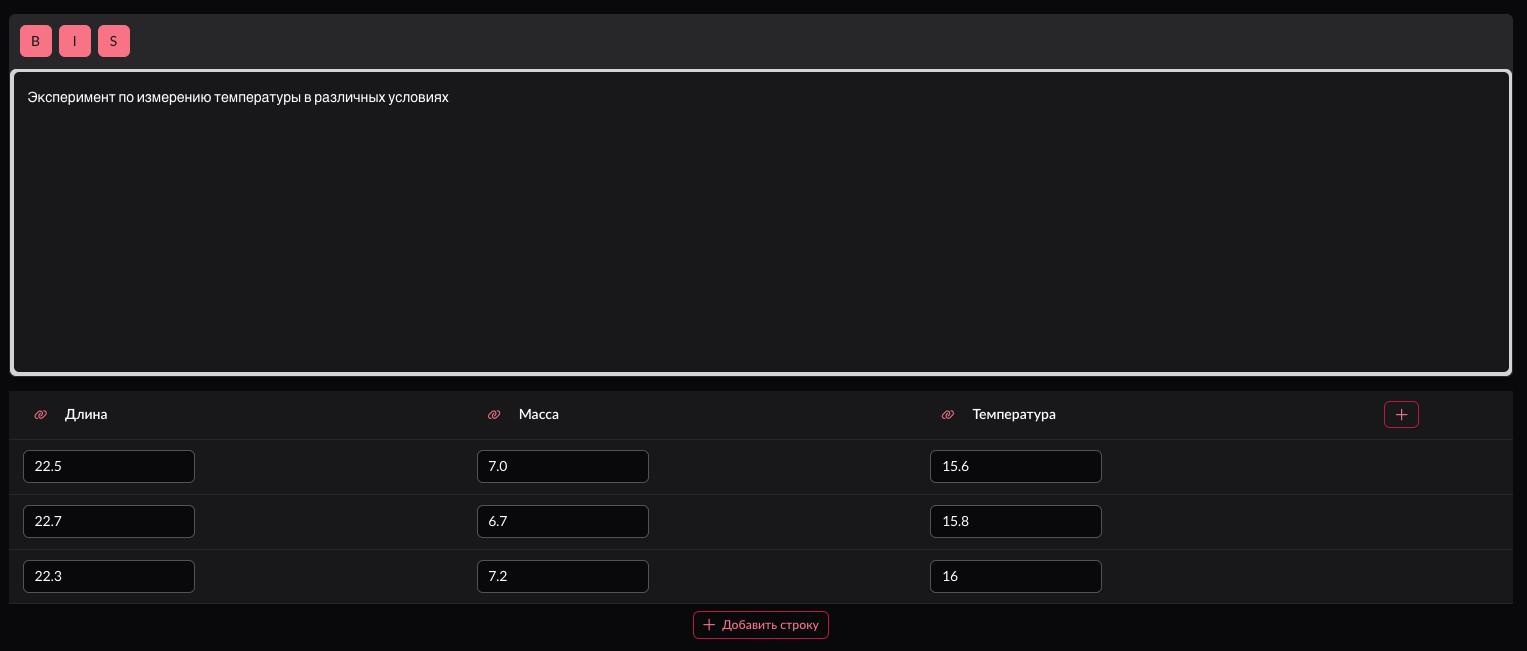
\includegraphics[width=\linewidth]{img/experiment_view.png}
\caption{Окно просмотра данных эксперимента}
\label{pic:lab_experiment_editor}
\end{figure}
\vspace{0.5cm}

\subsubsection{Таблица результатов измерений}

Таблица результатов измерений является важной частью экспериментов, позволяя пользователю фиксировать и анализировать полученные данные.
Каждая колонка таблицы может быть связана с определённой онтологией, что позволяет обеспечить корректную интерпретацию данных.

При редактировании эксперимента пользователь может задать для каждого столбца его онтологию и элемент онтологии, который этот столбец репрезентует.
Это облегчает обмен данными с другими системами.
Отображение таблицы реализовано в виде интерактивного компонента, который позволяет пользователям редактировать данные.

\subsubsection{Адаптивность и мобильная версия}

Интерфейс приложения адаптирован под мобильные устройства с использованием медиазапросов и классов Tailwind CSS (рис.~\ref{pic:mobile_version}).
Адаптивность обеспечивается настройками макета, темы, акцентного цвета и цвета фона (рис.~\ref{pic:other_colors}).

Благодаря этому при уменьшении ширины экрана боковая панель скрывается, а контент центрируется, а пользователи с особенностями зрения могут подобрать комфортное для них сочетание цветов и темы, делающее управляющие элементы сайта наиболее заметными, а работу комфортной.

\begin{figure}[H]
\centering
\begin{minipage}{0.45\linewidth}
\centering
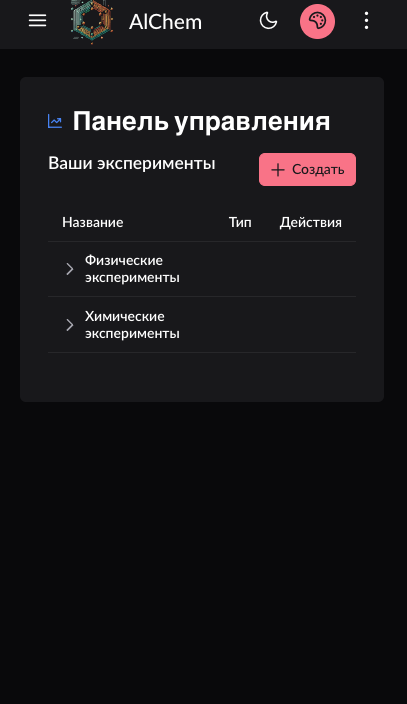
\includegraphics[width=\linewidth]{img/mobile_version.png}
\caption{Окно просмотра данных эксперимента}
\label{pic:mobile_version}
\end{minipage}\hfill
\begin{minipage}{0.45\linewidth}
\centering
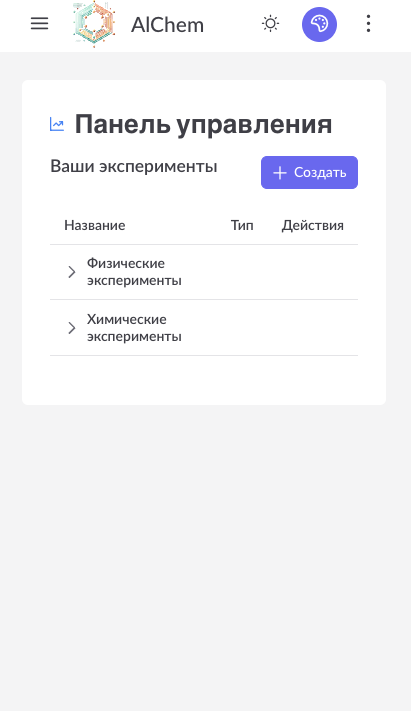
\includegraphics[width=\linewidth]{img/other_colors.png}
\caption{Выбор других сочетаний цветов и темы}
\label{pic:other_colors}
\end{minipage}
\end{figure}
\vspace{0.5cm}

\subsection{Работа с базой данных}

\subsubsection{Структура базы данных и схемы таблиц}

В качестве основной СУБД используется PostgreSQL, обеспечивающая высокую надёжность и поддержку сложных реляционных связей.
Схема базы данных (рис.~\ref{pic:postgres_scheme}) организована таким образом, чтобы минимизировать дублирование данных и оптимизировать запросы.

\begin{figure}[H]
\centering
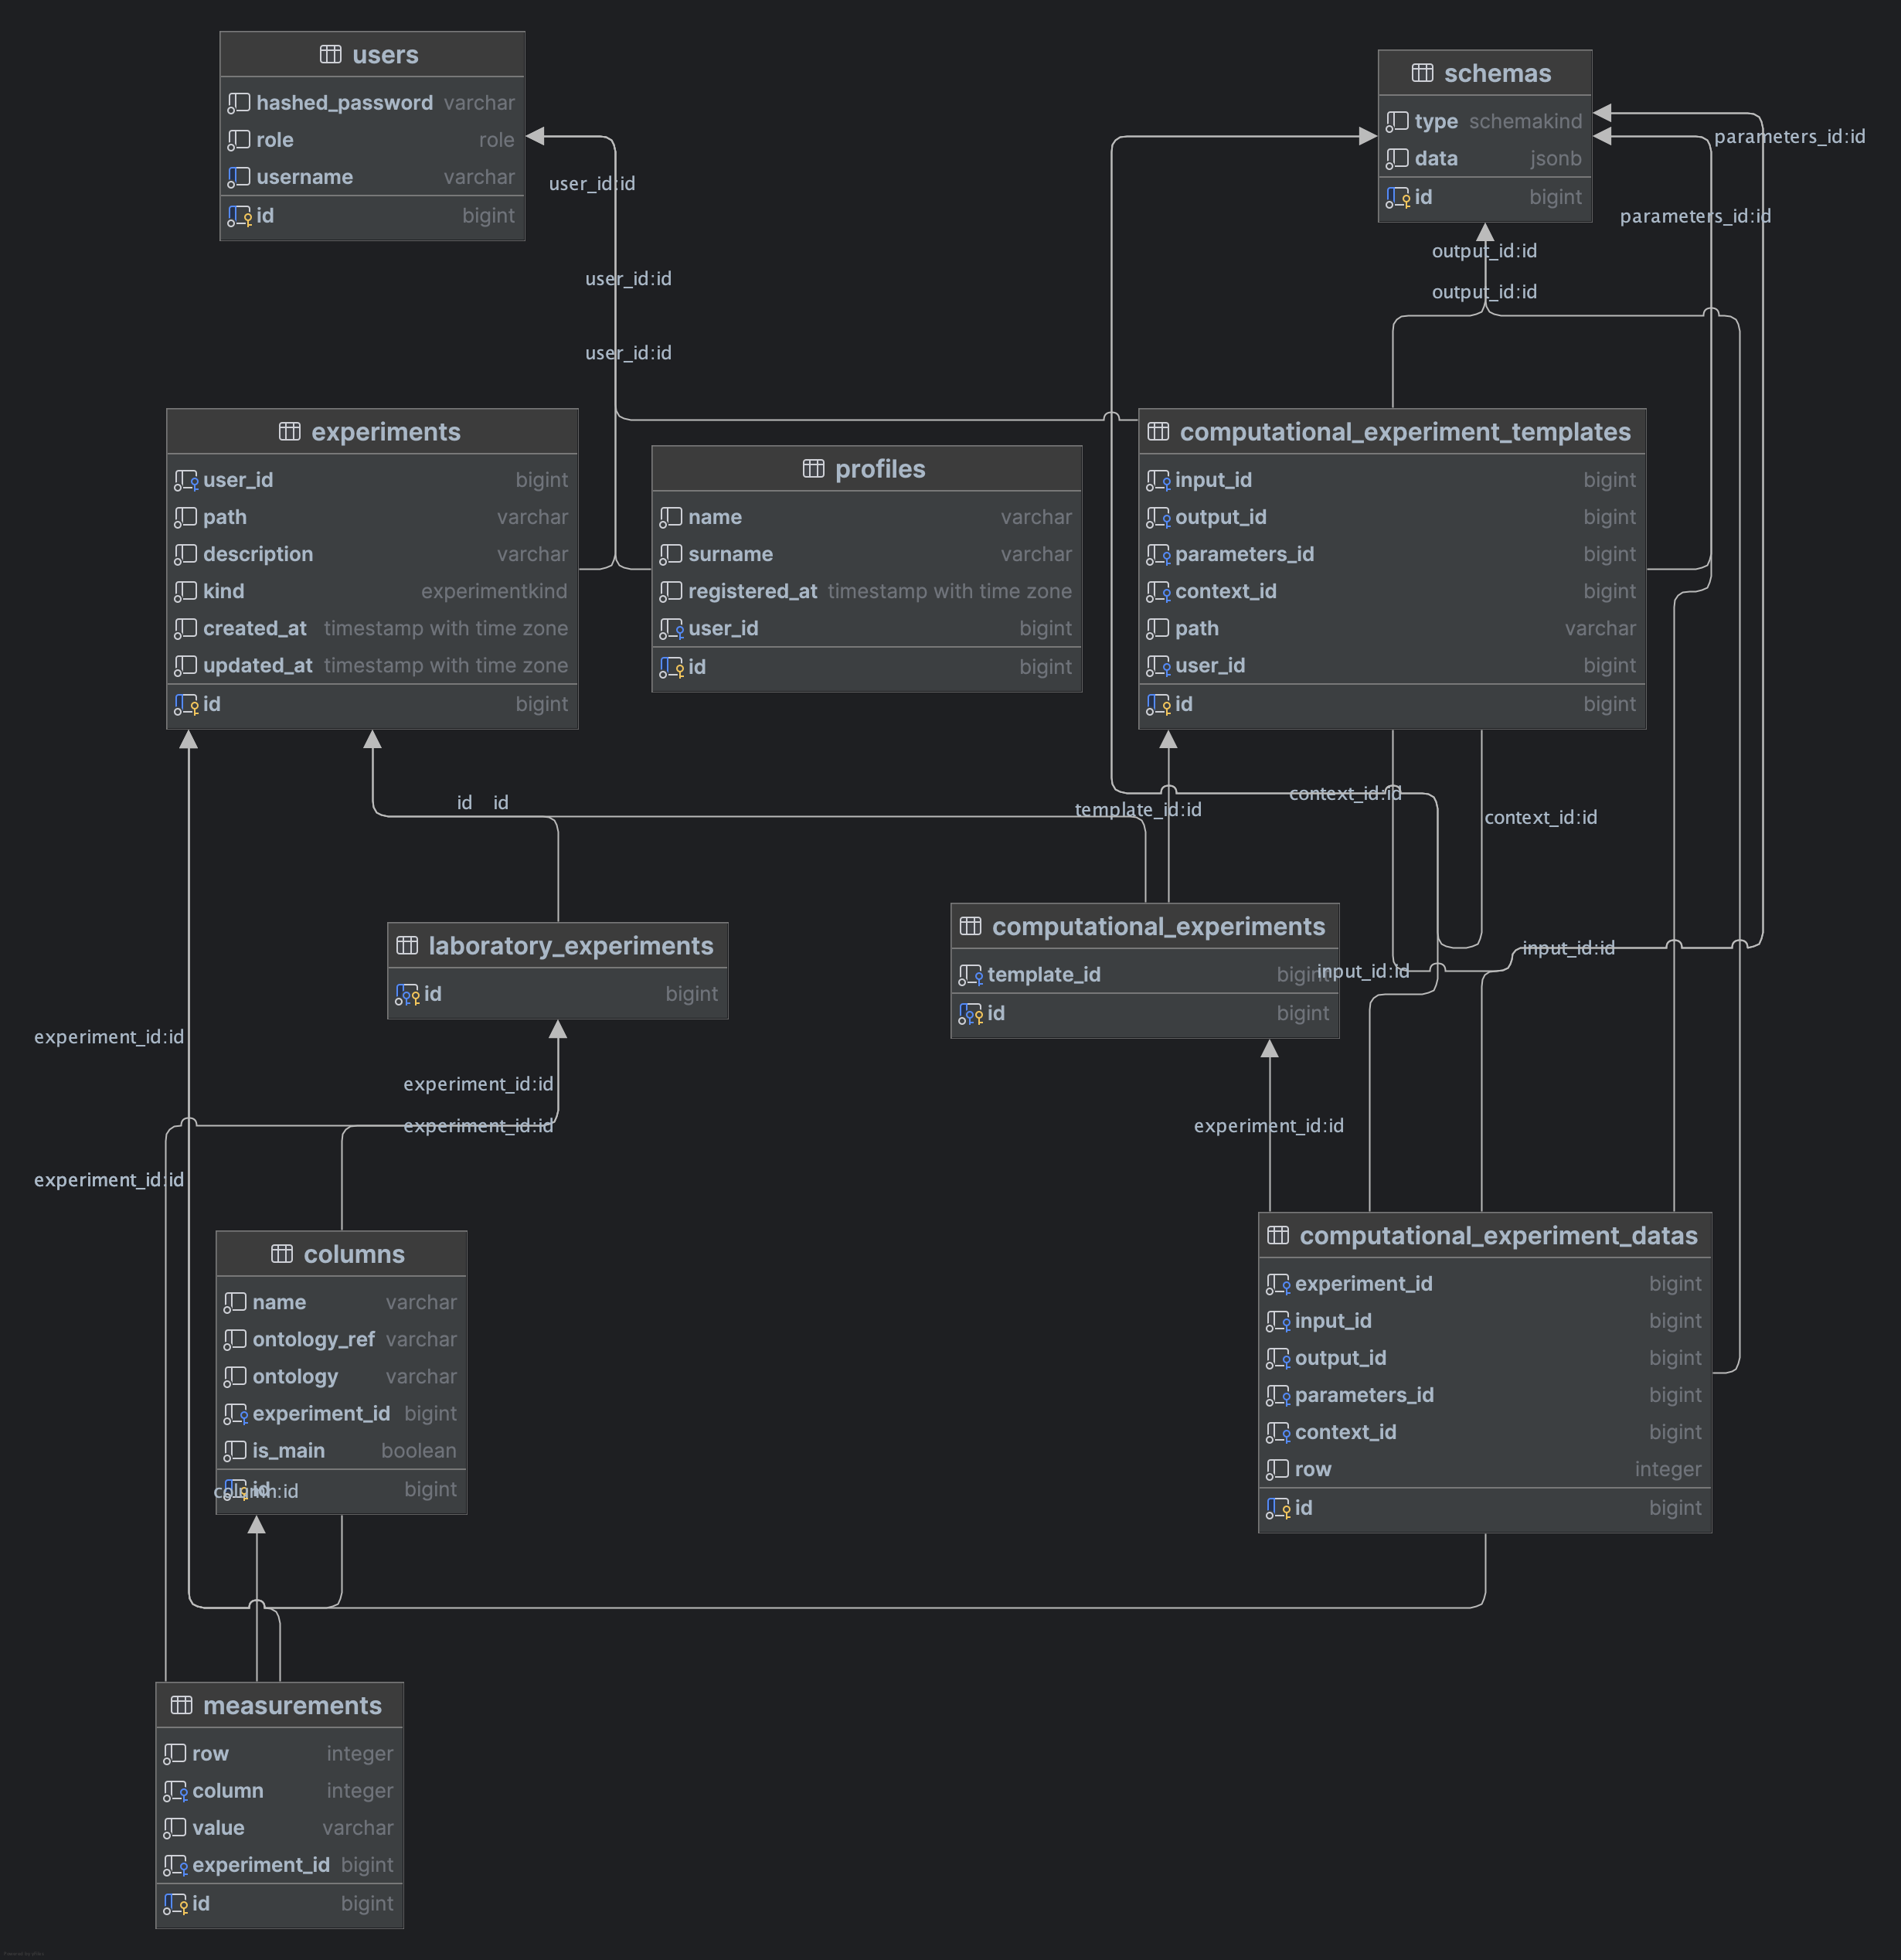
\includegraphics[width=\linewidth]{img/postgres_scheme.png}
\caption{Схема базы данных}
\label{pic:postgres_scheme}
\end{figure}
\vspace{0.5cm}

\subsubsection{ORM-модели}

Для работы с базой данных используется SQLAlchemy, обеспечивающая удобную работу с объектами и связями.
Модели представляют таблицы базы данных в виде классов, что позволяет писать гибкий и безопасный код.
ORM упрощает работу с базой, делает возможным автоматическое создание миграций для базы данных и сокращает количество SQL-запросов, оптимизируя их.

Основные сущности перечислены в~\ref{ORM models}.

\subsubsection{Управление миграциями}

Alembic используется для управления схемой базы данных, упрощая процесс обновления структуры данных без потери информации.
Среди возможностей этого инструмента особенно полезными можно назвать автоматическое создание миграций при изменении зарегистрированных моделей, возможность отката к предыдущим версиям схемы, и, как следствие, контроль изменений базы через версионирование.
Всё это позволяет плавно изменять схему базы, исключая конфликты данных.

\subsection{Интеграция с онтологиями}

\subsubsection{Способы привязки данных к онтологиям}

Каждый столбец таблицы измерений может быть связан с онтологией (рис.~\ref{pic:linked_to_ontology_column}), обеспечивая стандартную интерпретацию данных.
Связь осуществляется через указание для столбца псевдонима онтологии и элемента онтологии, зарегистрированной в приложении под этим псеводонимом.
Такое автоматизированное сопоставление данных снижает вероятность ошибок при интерпретации.

\begin{figure}[H]
\centering
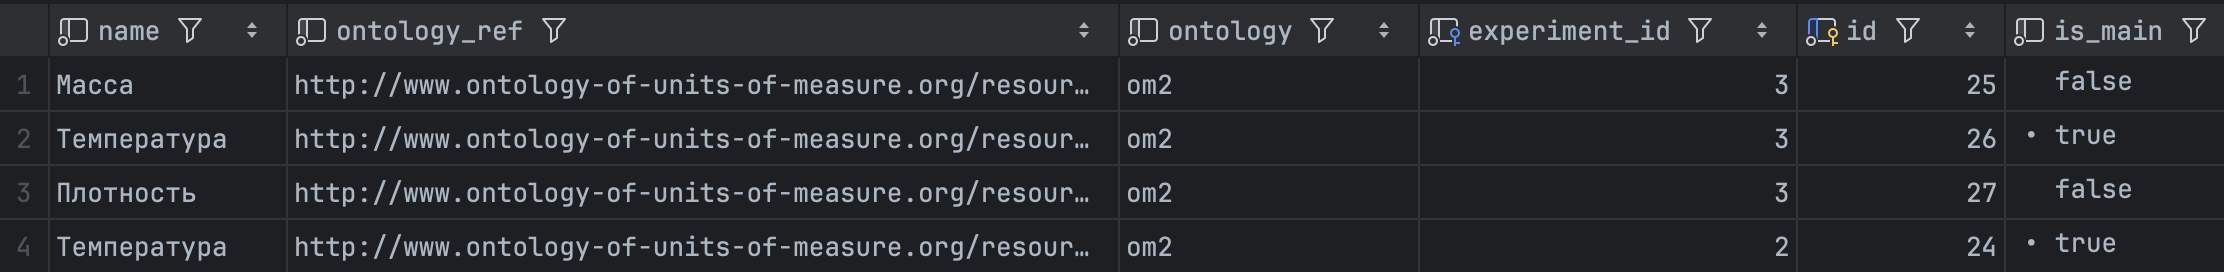
\includegraphics[width=\linewidth]{img/ontology_linking.png}
\caption{Столбец, привязанный к онтологии}
\label{pic:linked_to_ontology_column}
\end{figure}
\vspace{0.5cm}

\subsubsection{Поддерживаемые онтологии}

Приложение поддерживает две онтологии:
\begin{enumerate}
\item OM2 -- онтология физических величин и единиц измерения.
\item СhEBI -- онтология химических соединений.
\end{enumerate}

\subsubsection{Возможности расширения онтологической поддержки}

Система спроектирована таким образом, чтобы поддерживать подключение новых онтологий.
Добавление новых источников знаний требует лишь обновления базы данных, API и написания модуля со специфичными для онтологии запросами.

\subsection{Тестирование и отладка}

\subsubsection{Модульное тестирование серверной части}

Для тестирования серверной части используются unit-тесты (рис.~\ref{pic:backend_unit_tests}), написанные с использованием пакета pytest~\cite{Library:Pytest}, проверяющие корректность работы моделей, API и механизмов аутентификации.

\begin{figure}[H]
\centering
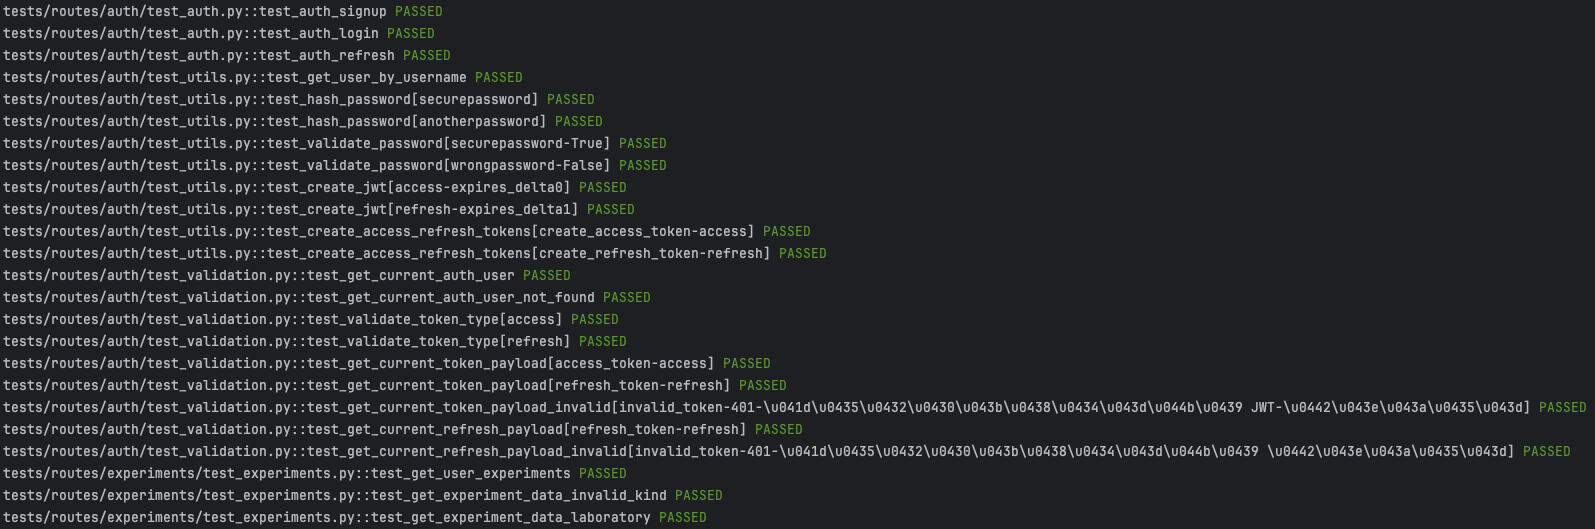
\includegraphics[width=\linewidth]{img/python_unit_tests.png}
\caption{Пример запуска unit-тестов серверной части}
\label{pic:backend_unit_tests}
\end{figure}
\vspace{0.5cm}

\subsubsection{Интеграционное тестирование API}

Для тестирования API применяется класс TestClient из FastAPI, который позволяет проверять работу маршрутов в изолированной среде.

% \subsubsection{Тестирование клиентской части}

% Фронтенд тестируется с помощью Cypress и Jest. Проверяются основные пользовательские сценарии: аутентификация, создание и редактирование экспериментов, работа с таблицами.

% \todo[inline]{Вставить пример теста интерфейса}

\subsection{Развёртывание и эксплуатация}

\subsubsection{Подготовка среды}

Приложение контейнеризовано с использованием Docker.
Все компоненты (серверная часть, клиентская часть, базы данных) запускаются через Docker Compose, обеспечивая предсказуемость окружения.
Это позволяет развернуть приложение на любом сервере без сложной настройки.
Также предусмотрены различные конфигурации Docker Compose, предназначенные специально для разработки, тестирования и продуктового окружения.

В продуктовом окружении приложение разворачивается с помощью Docker Compose, который управляет следующими сервисами:
\begin{enumerate}
\item backend -- контейнер с серверной частью.
\item frontend -- контейнер с обратным прокси-сервером для работы с клиентом.
\item db -- контейнер с PostgreSQL.
\item neo4j -- контейнер с Neo4j.
\end{enumerate}

\subsubsection{Настройка Nginx как обратного прокси}

Для маршрутизации запросов используется Nginx, который проксирует HTTP-запросы от фронтенда к бэкенду, а также управляет статическими файлами, что повышает общую производительность системы и отзывчивость для пользователя.

Основные настройки:
\begin{enumerate}
\item Проксирование API-запросов на бэкенд.
\item Кеширование статических файлов.
\end{enumerate}

\subsubsection{Запуск приложения}

Для запуска приложения необходимо предварительно заполнить конфигурационные файлы и воспользоваться системой контейнеризации Docker Compose.
Это обеспечивает воспроизводимость окружения и облегчает развёртывание как на локальной машине, так и на сервере.

\paragraph{Заполнение конфигурации} \mbox{}\\

Перед запуском требуется создать или отредактировать файлы переменных окружения для всех компонентов.
Для этого используются файлы \texttt{.env} в корне проекта и в директории \texttt{backend/config}.
В них указываются параметры подключения к базам данных, секретные ключи, настройки портов и прочие параметры.
Пример содержимого файла \texttt{.env} в листинге~\ref{lst:config_all}.
\begin{lstlisting}[frame=single, basicstyle=\footnotesize\ttfamily, label={lst:config_all}, caption={Заполнение конфигурационного файла всего приложения},captionpos=b, breaklines=true, breakatwhitespace=true, language=bash]
PG_USER=postgres
PG_PASSWORD=123
PG_DB=postgres

NEO4J_USER=neo4j
NEO4J_PASSWORD=123
\end{lstlisting}

Для запуска серверного приложения требуется создание в директории \texttt{backend/config} файла \texttt{config.stable.toml}, в котором нужно в формате TOML~\cite{Format:TOML} определить по крайней мере параметры \texttt{db.host}, \texttt{db.password}, \texttt{neo4j.host}, \texttt{neo4j.password}.
Также необходимо зарегистрировать онтологии по следующему принципу: секция \texttt{ontologies} представляет собой отображение, где ключ являются псевдонимом онтологий, которое затем может быть использовано в клиентском приложении, а значением – название метки, которая должна быть у каждого элемента онтологии.
Таким образом, если есть в секции \texttt{ontologies} пара, например, (OM2, om2UniqueLabel) приложение будет интерпретировать всякий результат запроса в Neo4j с меткой om2UniqueLabel как элемент онтологии OM2.

Пример содержимого файла \texttt{backend/config/config.stable.toml} в листинге~\ref{lst:config_backend}.
\begin{lstlisting}[frame=single, basicstyle=\footnotesize\ttfamily, label={lst:config_backend}, caption={Заполнение конфигурационного файла серверного приложения},captionpos=b, breaklines=true, breakatwhitespace=true]
[uvi]
host = ""
port = 0
workers = 0
timeout = 0
debug = false

[db]
port = 0
user = ""
database = ""
echo = false
echo_pool = false
pool_size = 0
max_overflow = 0
host = ""
password = ""

[neo4j]
port = 0
user = ""
db = ""
host = ""
password = ""

[jwt]
algorithm = ""
access_token_expire_minutes = 0
private_key_path = ""
public_key_path = ""
refresh_token_expire_minutes = 0

[ontologies]
OM2 = '__OntologyOM2__'
ChEBI = '__OntologyChEBI__'
\end{lstlisting}

\paragraph{Запуск с помощью Docker Compose} \mbox{}\\

После настройки переменных окружения приложение запускается одной командой: \texttt{docker-compose up --build}.
Эта команда соберёт и запустит все необходимые сервисы: серверную часть, клиентскую часть, базы данных PostgreSQL и Neo4j, а также Nginx для проксирования запросов.

Для запуска в фоновом режиме можно использовать флаг \texttt{-d}: \texttt{docker-compose up --build -d}

\paragraph{Дополнительные команды} \mbox{}\\

Для управления жизненным циклом приложения используются стандартные команды Docker Compose:
\begin{itemize}
\item Остановить сервисы: \texttt{docker-compose down}
\item Перезапустить сервисы: \texttt{docker-compose restart}
\item Просмотреть логи: \texttt{docker-compose logs -f}
\end{itemize}

\paragraph{Доступ к приложению} \mbox{}\\

После успешного запуска приложение становится доступно по адресу, указанному в настройках Nginx (по умолчанию \texttt{http://localhost/}).
Все компоненты приложения взаимодействуют друг с другом через внутреннюю сеть Docker Compose.

\anonsubsection{Выводы по главе}

В данной главе рассмотрена программная реализация веб-приложения, включая серверную и клиентскую части, работу с базой данных, интеграцию с онтологиями, тестирование и развёртывание. Архитектура приложения построена по клиент-серверной модели, обеспечивая высокую производительность и удобство работы с данными. Использование ORM упростило взаимодействие с базой данных, а поддержка онтологий позволила связывать экспериментальные данные с формализованными научными сущностями. Гибкое управление состоянием во фронтенде и система тестирования способствуют надёжности работы интерфейса и API. Развёртывание через контейнеризацию обеспечивает переносимость, а механизмы аутентификации и защиты данных гарантируют безопасность. В результате создана масштабируемая и расширяемая система для управления лабораторными и вычислительными экспериментами, адаптируемая к новым требованиям.